\section{All-\mask Block Already Knows}
\label{sec:motivation}
\begin{figure*}[t!]
    \centering
    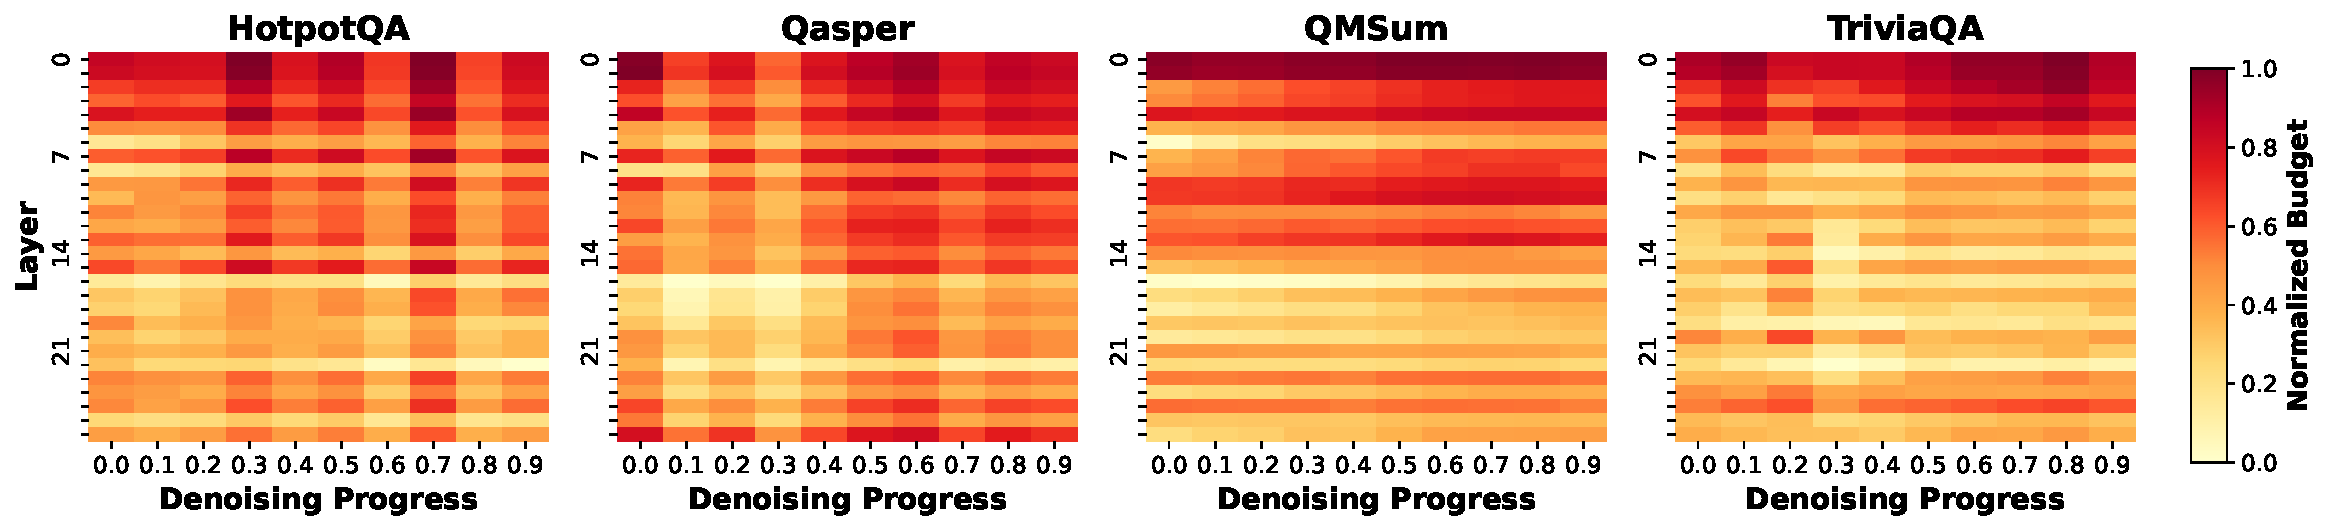
\includegraphics[width=\textwidth]{figures/fig4_sparsity_consistency_1x4.pdf}
    \caption{
    Layer-wise budget across denoising progress on four LongBench tasks. Color indicates normalized budget (darker = higher). Early layers require larger budgets, while horizontal bands indicate stable relative budgets throughout denoising.
    }
    \label{fig:sparsity_consistency}
\end{figure*}

In this section, we present a key observation that enables effective and efficient dynamic sparse attention for block diffusion LLMs. We find that the attention scores computed at the first denoising step, namely on the All-\mask block, already contains the signal needed to guide sparse attention throughout the subsequent denoising steps. Specifically, two pieces of information demonstrate temporal consistency across denoising steps within a block: (1) the top-K KV entries, and (2) attention score skewness.

\subsection{Consistent Top-K KV Entries}
\label{subsec:topk_consistency}

Each block begins as an All-\mask block and generates tokens through multiple denoising steps. At each step $t$, we compute the oracle top-K set $S_{\text{oracle}}^{(t)}$ via full attention. To measure how well the initial selection remains valid, we define the top-K recall rate at step $t$ as $|S_{\text{oracle}}^{(0)} \cap S_{\text{oracle}}^{(t)}| / K$: the fraction of step-0 selections that remain in the oracle set at step $t$. Figure~\ref{fig:topk_consistency} shows the top-K recall across denoising steps on four LongBench tasks. As denoising progresses, the recall gradually decreases but remains consistently high, with average values of 83.8\% for $K{=}512$, 86.2\% for $K{=}1024$, and 89.6\% for $K{=}2048$. These results indicate that the important context identified at the All-\mask step is largely preserved across denoising steps, enabling the All-\mask block to serve as a reliable guide for sparse attention in subsequent steps.

For comparison, we evaluate two representative sparse attention methods designed for AR LLMs, Quest~\cite{tang2024quest} and Tidal~\cite{yang2025tidaldecode}, adapted to block diffusion. We measure each method's top-K recall as $|S_{\text{method}} \cap S_{\text{oracle}}| / K$, where $S_{\text{method}}$ denotes the method's selected set and $S_{\text{oracle}}$ is the oracle set from full attention. As shown in Figure~\ref{fig:method_comparison}, Quest achieves 48--82\% recall via page-level importance estimation, while Tidal achieves 36--74\% by reusing anchor layer selections across other layers. All-\mask-guided selection achieves substantially higher recall (84--90\%) by leveraging the temporal consistency of attention patterns unique to block diffusion.
Intuitively, this consistency arises because the 
All-\mask block, despite lacking decoded token information, 
already captures the structural relevance patterns of the 
input context.


\subsection{Consistent Attention Score Skewness}
\label{subsec:budget_stability}
For dynamic sparse attention, determining how many KV entries to select in each layer is as important as identifying which KV entries are important. Layers exhibit different levels of attention-score skewness. Under a fixed total computation budget, it is beneficial to select fewer KV entries to more skewed layers and more KV entries to less skewed layers. Importantly, each layer’s skewness remains highly stable across denoising steps within a block.

Figure~\ref{fig:sparsity_consistency} visualizes the temporal consistency of layer-wise skewness within a block. As a proxy for skewness, we measure, for each layer, the number of KV entries required to reach 90\% attention coverage (the cumulative sum of attention scores after softmax), averaged over KV heads. Although skewness varies substantially across layers and tasks, it remains largely stable across denoising steps, as indicated by the horizontal band-like patterns in each heatmap. This stability suggests that skewness measured at the first denoising step can be reused to allocate layer-specific budgets throughout the entire denoising process.
